\chapter{Исследовательский раздел}

\section{Конфигурация экспериментального стенда}

Для проверки разработанного решения использован графический планшет XP-PEN Deco Fun L, подключённый кабелем USB Type-C. Производитель предусматривает проводное USB-подключение данной серии~\cite{tablet}. Стенд работает под управлением Ubuntu 24.04.3 ARM64 в виртуальной машине Parallels Desktop. Физическое USB-устройство передано гостевой системе целиком: одного преобразования движений в виртуальную мышь для проверки USB-драйвера недостаточно.

В таблице~\ref{tab:stand} приведены параметры, установленные по диагностике целевой системы. Все команды сборки и эксплуатации выполняются внутри Ubuntu из каталога проекта.

\begin{table}[htbp]
\caption{Параметры экспериментального стенда}
\label{tab:stand}
\centering\small
\begin{tabular}{|p{0.38\textwidth}|p{0.53\textwidth}|}\hline
Параметр & Значение \\ \hline
Устройство & XP-PEN Deco Fun L \\ \hline
USB VID:PID & \texttt{28bd:0932} \\ \hline
Гостевая ОС & Ubuntu 24.04.3 ARM64 \\ \hline
Версия ядра & \texttt{7.0.0-43-generic} \\ \hline
Архитектура & \texttt{aarch64} \\ \hline
Компилятор & GCC 13.3.0 \\ \hline
Транспорт & USB, полная скорость 12 Мбит/с \\ \hline
Входная конечная точка пера & \texttt{0x82}, interrupt IN \\ \hline
Максимальный пакет и интервал & 64 байта; 4 мс \\ \hline
Формат отчёта пера & Идентификатор 7; длина 10 байт \\ \hline
\end{tabular}
\end{table}

Вывод \texttt{lsusb} содержит строку \texttt{28bd:0932 XP-Pen 10 inch PenTablet}. В дереве USB обнаружены три HID-интерфейса. До переключения привязок они обслуживались транспортным драйвером \texttt{usbhid}; в sysfs обработчиком созданных HID-устройств являлся \texttt{hid-generic}. Интерфейс 0 создавал устройства совместимости мыши и клавиатуры, интерфейс 1 --- устройство пера, интерфейс 2 предоставлял вспомогательный обмен. Разработанный драйвер занимает первые два интерфейса, оставляя третий штатной подсистеме.

Аппаратная специализация реализации ограничена таблицей USB ID и форматом входного отчёта. Разъём Type-C не задаёт этот формат. Для другого планшета требуется отдельно проверить идентификаторы, интерфейсы, конечные точки и значения полей; добавление произвольного USB ID не обеспечивает совместимость.

\section{Проверка сборки и соответствия ядру}

Модуль собран средствами Kbuild с дополнительными предупреждениями \texttt{W=1}. Проверка выполнялась командами
\begin{lstlisting}[language=bash,basicstyle=\small\ttfamily]
make
modinfo -F vermagic ./xppen_mouse.ko
uname -r
\end{lstlisting}
В полученном выводе метаданные модуля имеют вид
\begin{lstlisting}[basicstyle=\footnotesize\ttfamily]
7.0.0-43-generic SMP preempt mod_unload modversions aarch64
\end{lstlisting}
а команда \texttt{uname -r} возвращает \texttt{7.0.0-43-generic}. Совпадение строки выпуска и архитектуры подтверждает сборку для целевого ядра. Само по себе оно не заменяет проверку поведения драйвера после загрузки.

Предупреждение о различии компиляторов связано с именами запуска \texttt{gcc-13} и \texttt{aarch64-linux-gnu-gcc-13}; в журнале обе версии указаны как GCC 13.3.0 одной сборки Ubuntu. Сообщение о пропуске BTF относится к отсутствию \texttt{vmlinux} при генерации отладочных метаданных. Завершение этапа линковки \texttt{xppen\_mouse.ko} показывает, что эти сообщения не остановили сборку.

\section{Результаты наблюдения событий ввода}

После загрузки модуля получен журнал утилиты \texttt{evtest}. Рассмотренный фрагмент начинается временной меткой 1794736999.199258 и заканчивается меткой 1794737019.447129; его продолжительность составляет 20,247871~с. В журнале присутствуют события \texttt{EV\_REL}, \texttt{EV\_KEY} и разделители \texttt{SYN\_REPORT}. Их смысл соответствует протоколу подсистемы ввода Linux~\cite{eventcodes}.

В первом пакете зарегистрированы \texttt{REL\_X=3} и \texttt{REL\_Y=-7}. Это задаёт приращение, а не абсолютную позицию на экране. В последующих пакетах встречаются положительные и отрицательные значения обеих осей. Отдельные пакеты содержат событие только одной оси: нулевое относительное перемещение не обязано передаваться потребителю. Траекторию указателя на экране по этим числам непосредственно определить нельзя, поскольку пользовательское окружение может применять собственную чувствительность и ускорение.

Для первых 12 пакетов движения интервалы между соседними временными метками находятся в диапазоне от 7,944 до 8,080~мс; среднее по 11 интервалам равно 8,00045~мс. Это характеристика выбранного участка выходного потока событий. Она не является измерением задержки от физического движения пера до экрана. Интервал обслуживания USB, равный 4~мс, также не означает обязательного появления нового события каждые 4~мс: устройство может формировать данные реже, а подсистема ввода не передаёт отсутствующие изменения.

В предоставленном журнале выделены пять пар нажатия и отпускания левой кнопки и четыре пары правой. В таблице~\ref{tab:button-observed} времена отсчитываются от первого события фрагмента, длительности вычислены как разность временных меток соответствующих \texttt{EV\_KEY}. Эти длительности описывают удержания кнопок, а не время обработки пакета драйвером.

\begin{table}[htbp]
\caption{Наблюдаемые циклы нажатия и отпускания кнопок}
\label{tab:button-observed}
\centering\small
\begin{tabular}{|p{0.25\textwidth}|p{0.27\textwidth}|p{0.29\textwidth}|}\hline
Кнопка & Начало, с & Удержание, мс \\ \hline
Левая, 1 & 1,431982 & 263,923 \\ \hline
Левая, 2 & 8,827967 & 2551,899 \\ \hline
Левая, 3 & 17,015859 & 1008,060 \\ \hline
Левая, 4 & 18,847956 & 87,921 \\ \hline
Левая, 5 & 19,783914 & 407,997 \\ \hline
Правая, 1 & 2,968030 & 151,994 \\ \hline
Правая, 2 & 4,343995 & 75,965 \\ \hline
Правая, 3 & 6,831899 & 136,066 \\ \hline
Правая, 4 & 7,967947 & 144,030 \\ \hline
\end{tabular}
\end{table}

Первое нажатие левой кнопки имеет метку 1794737000.631240, а отпускание --- 1794737000.895163. Между ними зарегистрировано относительное перемещение по оси Y. Аналогично между нажатием левой кнопки в 1794737008.027225 и отпусканием в 1794737010.579124 поступает последовательность относительных перемещений. Следовательно, поток событий сохраняет удержание кнопки во время движения и позволяет реализовать перетаскивание средствами пользовательского окружения.

На рисунке~\ref{fig:observed-buttons} показаны состояния кнопок, восстановленные по зарегистрированным переходам. Все девять наблюдаемых циклов завершены отпусканием. Это подтверждает корректное формирование обеих пар событий в рассмотренном фрагменте, но не характеризует обработку аварийного отключения USB.

\begin{figure}[htbp]
\centering
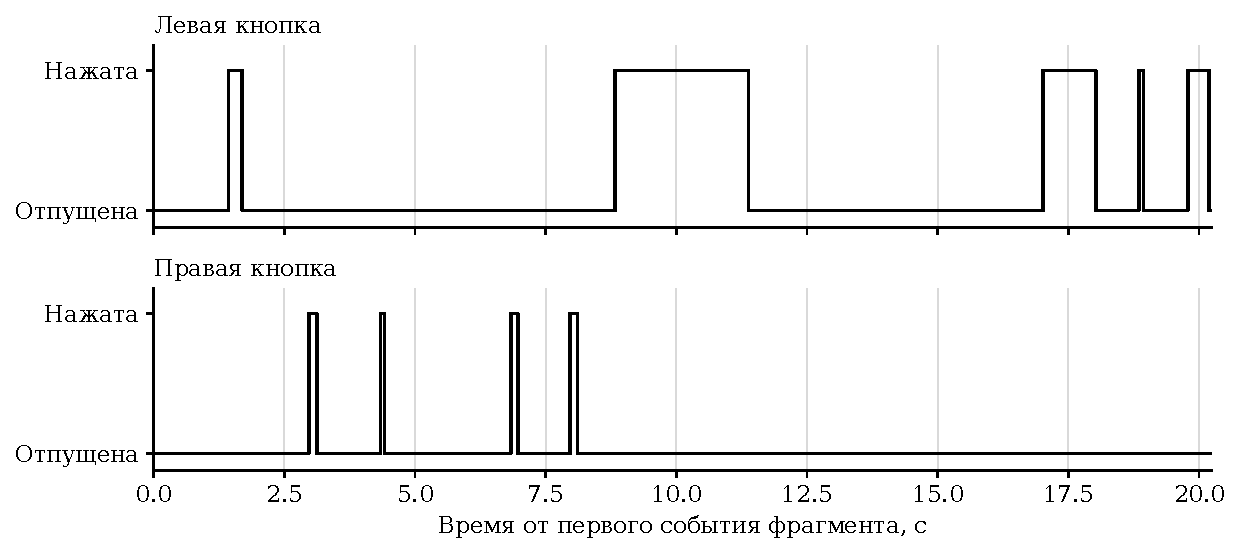
\includegraphics[width=\textwidth]{pdf/button_states.pdf}
\caption{Состояния кнопок по временным меткам журнала событий}
\label{fig:observed-buttons}
\end{figure}

\section{Расчётная проверка масштабирования перемещений}

Для отделения свойств алгоритма от настроек рабочего стола рассмотрена расчётная последовательность координат. Это численный пример применения формулы~\eqref{eq:relative-x}, а не измерение движения реального пера. При делителе $d=8$ и исходном положении $x_0=100$ результаты приведены в таблице~\ref{tab:remainder-example}.

\begin{table}[htbp]
\caption{Учёт малых перемещений при делителе 8}
\label{tab:remainder-example}
\centering\small
\begin{tabular}{|c|c|c|c|c|}\hline
Шаг & $x_k$ & $x_k-x_{k-1}$ & $\Delta x_k$ & $r_k$ \\ \hline
0 & 100 & --- & 0 & 0 \\ \hline
1 & 103 & 3 & 0 & 3 \\ \hline
2 & 106 & 3 & 0 & 6 \\ \hline
3 & 109 & 3 & 1 & 1 \\ \hline
4 & 110 & 1 & 0 & 2 \\ \hline
5 & 100 & $-10$ & $-1$ & 0 \\ \hline
\end{tabular}
\end{table}

Два первых смещения меньше делителя, однако их сумма не теряется. На третьем шаге накопленное значение равно 9 и формируется одна выходная единица. При возврате в исходную точку на пятом шаге накопленная величина равна $-8$, что даёт смещение $-1$ и нулевой остаток. Суммарное выходное смещение замкнутого движения равно нулю. Без сохранения остатков каждый положительный шаг этого примера был бы отброшен, а отрицательный дал бы $-1$, то есть возникла бы направленная ошибка.

Для одиночного исходного смещения 16 единиц делители 1, 2, 4, 8 и 16 дают соответственно 16, 8, 4, 2 и 1 выходную единицу. Увеличение делителя уменьшает чувствительность, но не изменяет назначения кнопок. В реализации допустимы значения от 1 до 1024; настройка выполняется при загрузке модуля. При выходе пера из зоны остатки сбрасываются вместе с началом отсчёта, поэтому накопление не связывает два независимых участка движения.

\section{Границы подтверждённых результатов}

Журнал подтверждает приём данных, формирование относительных событий, завершённые циклы обеих кнопок и движение при удержании левой кнопки. Проверка сборки подтверждает получение модуля для выбранного ядра. Корректность арифметики малых перемещений дополнительно показана расчётным примером.

Наблюдаемые записи не содержат отметок физических действий и не позволяют отдельно установить режим наведения, момент потери пера или задержку до отрисовки указателя. Для этих свойств требуется управляемый сценарий с фиксацией действий оператора. Также отдельно проверяются отключение USB при удержании кнопки, повторная привязка, выгрузка, suspend/resume и восстановление после ошибки конечной точки. В качестве критериев принимаются освобождение кнопок, отсутствие скачка при новом начале отсчёта, восстановление штатной обработки после выгрузки и отсутствие сообщений об ошибках обращения к памяти.

Таким образом, на выбранном стенде подтверждены основные выходные функции преобразования, а переносимость решения ограничена аппаратным профилем и совместимостью API целевого ядра. Результаты не распространяются автоматически на другие модели планшетов и на незафиксированные аварийные сценарии.
\clearpage
